% =====================================================================
% PP1 — DALI@MICCAI / medRxiv manuscript (Springer LNCS format)
% Generated from manuscript_claude.md. Compile on Overleaf with the
% LNCS (llncs) template. AUTHOR PLACEHOLDER — fill before submission.
% =====================================================================
\documentclass[runningheads]{llncs}

\usepackage[T1]{fontenc}
\usepackage{graphicx}
\usepackage{booktabs}
\usepackage{amsmath}
\usepackage{amssymb}
\usepackage{multirow}
\usepackage{url}

\begin{document}

\title{Cross-Population Generalization of Proxy-Trained Chest X-Ray Models for Tuberculosis: A Specialist Fails on the Target MENA Population Where a Zero-Shot Foundation Model Succeeds}
% \subtitle{}

\author{Adem Sahli\orcidID{0009-0003-0749-0575}}
\institute{Higher Institute of Computer Science (ISI), Tunisia \\
\email{sahliadem0106@gmail.com} \\
\url{https://github.com/sahliadem0106/pp1-tb-crosspopulation}
}

\maketitle

\begin{abstract}
Tuberculosis remains a leading cause of death, and automated chest radiography screening is a promising tool for high-burden and underserved regions, including the Middle East and North Africa (MENA). Whether such models generalize across populations is largely untested. We trained a DenseNet-121 on NIH ChestX-ray14 using the Infiltration finding as a proxy for tuberculosis and evaluated the frozen model on three external datasets: Montgomery (USA), Shenzhen (China), and a MENA dataset from Qatar. The model transferred unevenly---matching or beating its home score on Shenzhen (AUC 0.769 vs.\ 0.715) but collapsing to near chance on Qatar (AUC 0.571, confidence interval disjoint from all others)---and at the WHO-recommended sensitivity of 0.90, specificity was unusably low on every dataset (0.11--0.38).

We probed the mechanism of this failure. Grad-CAM revealed the specialist's decisions rest on a stereotyped right-upper-lung spatial prior whose attention collapses to image background on errors, and UMAP showed the target population is \emph{not} out-of-distribution in feature space---indicating a decision-process artifact rather than distribution shift. Consistent with this, a zero-shot foundation model (BiomedCLIP) succeeded on the same Qatar images (AUC 0.838, artifact-controlled) with +0.267 over the fine-tuned specialist. We conclude that cross-population failure in proxy-trained TB models is driven by shortcut-like decision processes, and that shortcut-robust foundation-model representations offer a promising path toward population-invariant TB screening.

\keywords{Tuberculosis screening \and chest radiography \and cross-population generalization \and shortcut learning \and foundation models \and Grad-CAM}
\end{abstract}

\clearpage

% ---------------------------------------------------------------------
% Teaser / pipeline figure (Figure 1)
% ---------------------------------------------------------------------
\begin{figure}[t!]
\centering
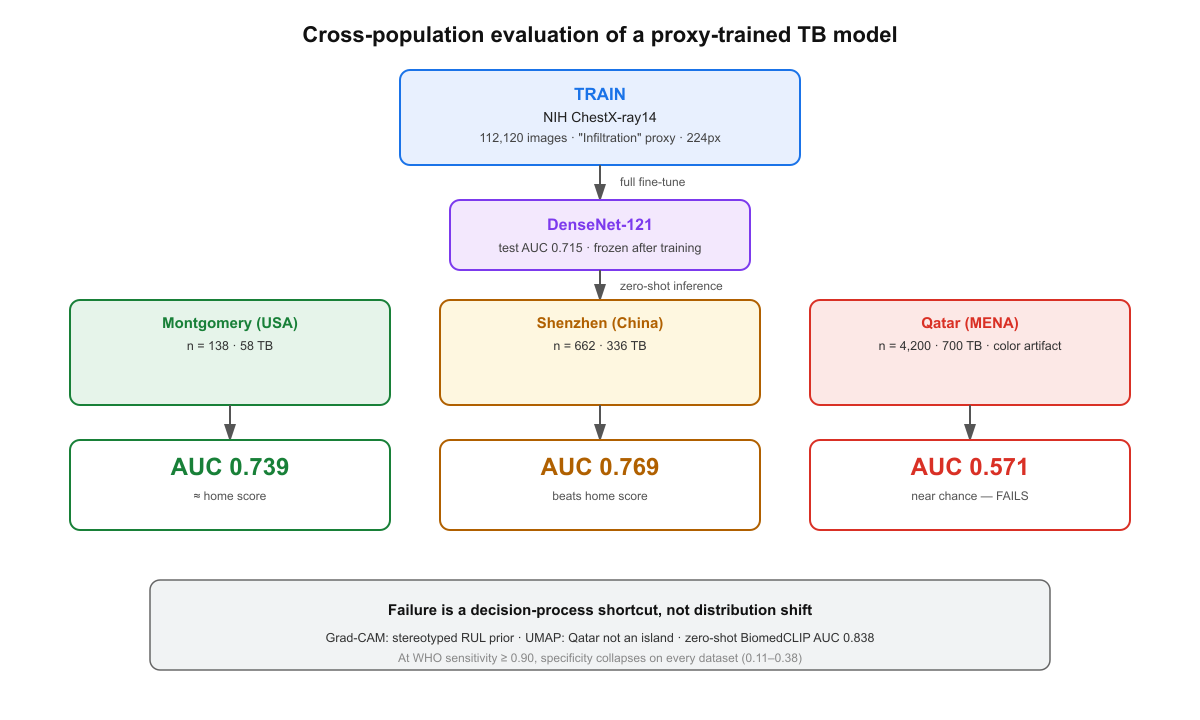
\includegraphics[width=\textwidth]{pipeline_figure}
\caption{Study design. A DenseNet-121 is trained on the NIH ChestX-ray14 Infiltration proxy and evaluated frozen on three external populations (Montgomery, Shenzhen, Qatar). The model transfers unevenly and fails on the MENA cohort; the failure is a decision-process shortcut, not distribution shift.}
\label{fig:pipeline}
\end{figure}

% ---------------------------------------------------------------------
\section{Introduction}
% ---------------------------------------------------------------------
Tuberculosis remains one of the world's deadliest infectious diseases. In 2024, the WHO estimated 10.7 million new cases and 1.23 million deaths, with the largest burden concentrated in low- and middle-income regions \cite{who2025}. The Middle East and North Africa (MENA) is increasingly recognized as a region of concern, where case detection gaps and rising drug resistance make reliable screening a priority \cite{whoemro2025}. Chest radiography is a first-line screening tool, and deep learning has raised the prospect of automated, low-cost TB screening in exactly these resource-constrained settings.

Yet a fundamental question remains largely unanswered: \emph{do chest X-ray models generalize across populations?} Most deep-learning TB systems are trained and evaluated on a single population, frequently the one that produced the training data. When such a model is deployed on a different population---different scanner, different acquisition protocol, different disease presentation, and different demographic makeup---its performance is not guaranteed to transfer. For a screening tool aimed at populations unlike its training cohort, this uncertainty is not a technical detail; it is a safety and deployment concern.

We investigate this question through a controlled cross-population evaluation of a tuberculosis model. We train a single DenseNet-121 on the NIH ChestX-ray14 dataset using the Infiltration finding as a proxy label for tuberculosis, then evaluate the frozen model on three external datasets: Montgomery (USA), Shenzhen (China), and a MENA dataset from Qatar. We further ask \emph{why} the model succeeds or fails, using Grad-CAM interpretability and representation-space analysis, and we compare the specialist against a large zero-shot foundation model (BiomedCLIP).

Our central finding is that the model's failure on the target MENA population is \emph{not a simple distribution-shift failure}: its decision process relies on a coarse, shortcut-like spatial prior, and a zero-shot foundation model that lacks that prior succeeds on the same images. These results suggest that cross-population generalization for TB screening is governed less by whether the data is ``in distribution'' and more by \emph{how the model decides}---and that foundation-model representations, free of proxy-label shortcuts, offer a promising path toward deployable, population-invariant TB screening.

\subsection*{Contributions}
\begin{itemize}
\item A controlled cross-population evaluation of a proxy-trained TB model on three external populations, including a MENA cohort (Table~\ref{tab:table1}), with statistical significance and WHO-operating-point analysis.
\item An interpretability and representation analysis showing the failure is decision-process-mediated (stereotyped spatial prior; attention collapse on errors; no representation-space separation).
\item A head-to-head zero-shot foundation-model comparison in which BiomedCLIP beats the fine-tuned specialist on the target population by +0.267 AUC, artifact-controlled.
\end{itemize}

% ---------------------------------------------------------------------
\section{Related Work}
% ---------------------------------------------------------------------
\subsection{AI for tuberculosis screening from chest radiographs}
Deep learning has repeatedly been shown to detect chest X-ray abnormalities at radiologist-competitive levels \cite{rajpurkar2017,irvin2019,wang2017}. For tuberculosis specifically, several systems report high accuracy on single-population cohorts and are promoted for screening in high-burden settings \cite{murphy2020}. A recurrent methodological caveat is that many of these systems are trained and evaluated on the \emph{same} population, leaving cross-population generalization---the property that matters for deployment---largely untested \cite{rajpurkar2020}.

\subsection{Cross-population generalization and distribution shift in medical imaging}
Medical imaging models are known to degrade under distribution shift---differences in scanner, acquisition protocol, population demographics, and disease presentation between training and deployment cohorts \cite{su2024}. A common finding is that models trained on one institution's data underperform on others', with performance drops that are difficult to predict a priori \cite{rajpurkar2020}. We add a MENA-targeted cross-population evaluation and probe the \emph{mechanism} of failure rather than reporting accuracy degradation alone.

\subsection{Shortcut learning and dataset bias}
Deep classifiers frequently rely on spurious correlations---``shortcuts''---rather than the medically meaningful signal: patient-position laterality markers, scan overlays, or acquisition-specific color and texture biases \cite{geirhos2020,zech2018}. Such shortcuts inflate within-distribution accuracy and silently break under shift \cite{geirhos2020}. Our Grad-CAM and representation analyses ask whether the observed cross-population failure is a consequence of shortcut-dependent decision processes rather than data being out-of-distribution.

\subsection{Foundation models and zero-shot transfer for medical imaging}
Contrastive image-text foundation models pretrained on large biomedical corpora (BiomedCLIP, ~15M image-text pairs) transfer to downstream tasks with little or no task-specific training \cite{zhang2023}. A key open question is whether such generalist models generalize across populations better than task-specialists fine-tuned on proxy-labeled data; we address this directly below.

% ---------------------------------------------------------------------
\section{Methods}
% ---------------------------------------------------------------------
\subsection{Datasets}
\textbf{Training set---NIH ChestX-ray14.} We trained on the NIH ChestX-ray14 dataset (112,120 frontal chest radiographs) using the \emph{Infiltration} finding as a proxy label for tuberculosis, following the CheXNet protocol \cite{rajpurkar2017}. Because NIH provides no TB-specific labels, we defined the positive class as images whose multi-label finding vector contained \emph{Infiltration} and the negative class as images labeled \emph{No Finding}. Images with other finding combinations were excluded, yielding 19,870 positive and 60,412 negative images (ratio $\approx$ 1:3.0). Images were resized to 224$\times$224 pixels.

\textbf{External test sets.} Three publicly available TB datasets were used for zero-shot external evaluation, none of which was used for training:
\begin{itemize}
\item \textbf{Montgomery} (USA; $n=138$; 80 normal / 58 TB)---Montgomery County Department of Health and Human Services.
\item \textbf{Shenzhen} (China; $n=662$; 326 normal / 336 TB)---Shenzhen No.~3 People's Hospital.
\item \textbf{Qatar TB} (MENA; $n=4{,}200$; 3,500 normal / 700 TB)---assembled at Hamad Medical Corporation (Doha, Qatar), used as a MENA-population proxy. This dataset carries a known acquisition artifact: a portion of the tuberculosis subset is colorized while the normal subset is uniformly grayscale. As detailed below, we evaluate on this set with color cues removed.
\end{itemize}
External dataset labels were encoded either in the filename suffix (Montgomery/Shenzhen: \texttt{\_0} = normal, \texttt{\_1} = TB) or in the directory structure (Qatar: \texttt{Normal/} vs \texttt{Tuberculosis/}). We generated per-dataset label manifests (CSV) from these encodings and verified the resulting class counts against the published dataset sizes before evaluation.

\subsection{Preprocessing}
All images were converted to grayscale and resized to 224$\times$224. For the DenseNet input we replicated the grayscale channel to three channels and applied the ImageNet normalization (mean = [0.485, 0.456, 0.406], std = [0.229, 0.224, 0.225]). During training only, a random horizontal flip was applied; the external-evaluation transform contained no augmentation and was identical to the training-set evaluation transform, ensuring a fair comparison across populations.

\subsection{Model and training}
\textbf{Architecture.} We fine-tuned a DenseNet-121 initialized with ImageNet weights; the classification head was replaced with a single linear unit producing a logit for the Infiltration proxy (BCE). All $\sim$7.0M parameters were trainable (full fine-tune).

\textbf{Training protocol.} NIH images were split \emph{patient-wise} (70/15/15) by stratified assignment of unique patient identifiers, preventing patient leakage between train, development, and test. Training minimized binary-cross-entropy-with-logits with class re-weighting ($\mathrm{pos\_weight} = n_{neg}/n_{pos} \approx 3.04$) to counter the $\sim$1:3 imbalance, using AdamW (lr $=10^{-4}$, weight decay $=10^{-4}$), a cosine annealing schedule ($T_{max}=25$), gradient clipping (max norm $=1.0$), and early stopping (patience $=6$ epochs) by development-set AUC. The best checkpoint by development AUC was retained. Seeds were fixed across Python, NumPy, and torch RNGs for reproducibility.

\subsection{Evaluation}
\textbf{Frozen inference.} The trained model was evaluated in evaluation mode with gradients disabled on the held-out NIH test split and on each external dataset. Per image we recorded the sigmoid probability of the positive class.

\textbf{Metrics.} For each dataset we computed the area under the ROC curve (AUC) using a pure-PyTorch rank computation, and precision, recall, and F1 at a 0.5 threshold. 95\% confidence intervals (CIs) for AUC were obtained by bootstrap resampling ($n=200$ replicates).

\textbf{WHO operating-point analysis.} Because tuberculosis screening tools are required to achieve high sensitivity, we determined, for each dataset, the highest decision threshold at which sensitivity $\geq 0.90$ and report the corresponding specificity and precision. This mirrors the WHO-recommended screening sensitivity target and is the clinically meaningful operating point.

\textbf{Statistical significance.} Differences between dataset AUCs were assessed via bootstrap confidence intervals on the AUC difference (AUC$_{NIH} - $AUC$_{external}$); a difference was deemed significant when its 95\% CI excluded zero.

\subsection{Interpretability---Grad-CAM}
To examine which image regions drove the model's decisions, we computed gradient-weighted class activation maps (Grad-CAM) \cite{selvaraju2017} from the final convolutional feature map of the DenseNet (7$\times$7). For each of Montgomery and Shenzhen we selected 10 true positives and 10 false negatives (at threshold 0.5). Heatmaps were upsampled to 224$\times$224, rectified, min-max normalized, and blended at 50\% opacity over the input. For a subset of false negatives we additionally inspected raw (un-normalized) activation magnitudes to rule out rescaling artifacts. The backward hook was registered on the output tensor to avoid the in-place-ReLU autograd conflict in DenseNet.

\subsection{Foundation-model comparison}
We compared the fine-tuned specialist against a large biomedical foundation model, BiomedCLIP (400M parameters; pretrained on $\sim$15M biomedical image-text pairs), used \emph{zero-shot}: images were scored by cosine similarity between the image embedding and the text prompts ``a chest x-ray showing infiltration'' and ``a chest x-ray showing no abnormality'', followed by a softmax over the two prompts. AUC was computed from the infiltration-prompt probability. Because the Qatar dataset contains a color acquisition artifact and BiomedCLIP accepts RGB input, we additionally re-evaluated Qatar with color cues removed (grayscale input), so the foundation-model comparison controls for the same artifact neutralized in the DenseNet pipeline.

\subsection{Implementation}
Experiments were run in PyTorch on an NVIDIA T4 GPU. External datasets were obtained from their public repositories; the model, data-processing, and evaluation code is available in the project repository. All AUC, threshold, and significance computations were implemented in pure PyTorch without reliance on scikit-learn.

% ---------------------------------------------------------------------
\section{Results}
% ---------------------------------------------------------------------
\subsection{Home held-out performance}
The fine-tuned DenseNet achieved a test AUC of \textbf{0.715} (95\% CI [0.707, 0.725]) on the held-out NIH test split ($n=17{,}260$; 3,016 positives / 14,244 negatives), with precision 0.313, recall 0.574, and F1 0.405 at a 0.5 threshold. This is consistent with prior reports for the Infiltration-vs-No-Finding proxy \cite{wang2017,rajpurkar2017}.

\subsection{Cross-population external evaluation}
Evaluated frozen on the three external datasets, the model transferred \emph{unevenly}. Table~\ref{tab:table1} summarizes the results.

\begin{table}[t]
\centering
\caption{Cross-population external evaluation of the NIH-trained DenseNet-121, evaluated frozen on the held-out NIH test split and three external datasets. AUC = area under the ROC curve; CI = 95\% bootstrap confidence interval; P/R/F1 = precision/recall/F1 at a fixed 0.5 threshold; WHO thr/sens/spec = threshold, sensitivity, and specificity at the WHO operating point (sensitivity $\geq 0.90$).}
\label{tab:table1}
\begin{tabular}{lrrrrrrrrr}
\toprule
Dataset & $n$ & AUC & CI & P & R & F1 & WHO$_{thr}$ & WHO$_{sens}$ & WHO$_{spec}$ \\
\midrule
NIH (home) & 17,260 & 0.715 & [0.707,0.725] & 0.313 & 0.574 & 0.405 & 0.203 & 0.900 & 0.320 \\
Montgomery & 138 & 0.739 & [0.650,0.813] & 0.917 & 0.190 & 0.314 & 0.065 & 0.914 & 0.112 \\
Shenzhen & 662 & 0.769 & [0.734,0.802] & 0.882 & 0.199 & 0.325 & 0.073 & 0.902 & 0.383 \\
Qatar (MENA) & 4,200 & 0.571 & [0.546,0.594] & 0.230 & 0.319 & 0.267 & 0.088 & 0.903 & 0.139 \\
\bottomrule
\end{tabular}
\end{table}

Two striking patterns emerge. First, on two of the three external populations the model performed at or above its home score: Shenzhen (AUC 0.769) was significantly higher than NIH (bootstrap difference CI [$-0.093$, $-0.020$]), and Montgomery (0.739) was comparable but noisier given its small size (CI crosses zero). That a model trained on NLP-derived proxy labels generalizes to \emph{real} TB cases on two populations---despite different scanners, populations, and countries---is a positive-transfer result.

Second, the model \emph{failed on the MENA dataset}: Qatar AUC was 0.571, near chance and statistically well below every other dataset (vs.\ NIH, difference CI [$+0.116$, $+0.170$]). The Qatar confidence interval [0.546, 0.594] is fully disjoint from all others.

\textbf{WHO-operability failure.} At the WHO-recommended screening sensitivity ($\geq 0.90$), specificity collapsed on \emph{every} dataset, including the home set: 0.320 (NIH), 0.112 (Montgomery), 0.383 (Shenzhen), and 0.139 (Qatar). The thresholds required to reach 90\% sensitivity were very low (0.065--0.203), meaning the model effectively labels any image with measurable signal as positive. No dataset could be screened at WHO sensitivity without referring roughly 62--89\% of healthy patients.

\begin{figure}[t]
\centering

\includegraphics[width=0.85\textwidth]{roc_overlay}
\caption{ROC curves for the NIH-trained DenseNet-121 on the held-out NIH test split and the three external datasets (AUC values as in Table~\ref{tab:table1}); the diagonal line marks chance performance (AUC = 0.5).}
\label{fig:roc}
\end{figure}

\subsection{What the model attends to (Grad-CAM)}
Grad-CAM on true positives from both external datasets showed attention concentrated within the lung parenchyma, with no reliance on corner markers, laterality text, or image borders---ruling out the most blatant burned-in-annotation shortcut. However, the highlighted region was \emph{stereotyped}: near-identical size, shape, and right-upper/mid-lung position across patients. Right-upper-lobe involvement is the most common presentation of post-primary TB, so this pattern is consistent with a coarse, epidemiologically plausible spatial prior---but not with lesion-specific localization, since the fixed geometry across patients suggests the model weights a lung region rather than detecting discrete pathology.

False negatives exhibited \emph{two distinct failure mechanisms}: (i) attention collapsing \emph{outside} the lungs (most often a horizontal bottom-border band, and in some cases a shoulder hotspot), and (ii) lung-region activation that was present and anatomically plausible but too weak to cross the 0.5 threshold (borderline-confidence failure). Raw (un-normalized) activation magnitudes confirmed that the border response was genuine rather than a min-max rescaling artifact; a modest border response ($\approx$ 8--11\% of peak activation) was present in all false negatives examined and became dominant when lung evidence was weak.

\begin{figure}[t]
\centering
\includegraphics[width=\textwidth]{gradcam_figure2_FULL}
\caption{Grad-CAM overlays for the NIH-trained specialist on Montgomery and Shenzhen true positives and false negatives (10 images per panel, threshold 0.5; heatmaps min-max normalized and blended at 50\% opacity over the input). A minority of false negatives (e.g., Montgomery \#9, Shenzhen \#2) exhibit no positive activation at all---raw activation magnitudes confirmed these cases are genuine near-zero maps rather than rendering artifacts, consistent with an absence of learned evidence for these images.}
\label{fig:gradcam}
\end{figure}

\subsection{A zero-shot foundation model succeeds where the specialist fails}
Using BiomedCLIP zero-shot (no training, text-prompt scoring), we compared the foundation model against the fine-tuned specialist (Table~\ref{tab:table2}).

\begin{table}[t]
\centering
\caption{Zero-shot BiomedCLIP versus the fine-tuned DenseNet-121 across all four evaluation sets. Qatar's BiomedCLIP AUC (0.838) uses color-neutralized (grayscale) input to control for a known acquisition artifact in the Qatar dataset's tuberculosis subset; the same images scored with the original RGB input give AUC 0.849 ($\Delta=0.011$), reported as a robustness check, not as the headline number.}
\label{tab:table2}
\begin{tabular}{lcc}
\toprule
Dataset & DenseNet (fine-tuned) & BiomedCLIP (zero-shot) \\
\midrule
NIH & 0.715 & 0.633 \\
Montgomery & 0.739 & \textbf{0.850} \\
Shenzhen & \textbf{0.769} & 0.650 \\
Qatar (MENA) & 0.571 & \textbf{0.838} (color-neutralized) \\
\bottomrule
\end{tabular}
\end{table}

The result is striking and \emph{artifact-controlled}: on the target MENA population, a foundation model with zero training achieved AUC \textbf{0.838}---a +0.267 gain over the fine-tuned specialist---and this held after color cues were removed from the Qatar input (0.838 vs.\ 0.849 with color, $\Delta = 0.011$). No single model wins everywhere (the specialist retains NIH and Shenzhen), but on the population of clinical interest, the generalist wins decisively.

\subsection{Representation geometry (UMAP)}
UMAP projections of the DenseNet features colored by dataset formed a single continuous manifold with no hard boundaries; \emph{Qatar was not an island} but overlapped extensively with NIH. The same overlap held in BiomedCLIP feature space, where Montgomery and Shenzhen formed distinct sub-clusters. This indicates the Qatar failure is \emph{not} attributable to gross out-of-distribution separation of the data---consistent with a decision-process explanation rather than a representation-space one.

\begin{figure}[t]
\centering

\includegraphics[width=0.95\textwidth]{umap_comparison}
\caption{UMAP projections of 1,024-dimensional image embeddings from the trained DenseNet-121 (left) and zero-shot BiomedCLIP (right), colored by source dataset. Qatar overlaps extensively with NIH in both representation spaces, while Montgomery and Shenzhen form more distinct sub-clusters under BiomedCLIP; cluster overlap and separation are descriptive of local embedding structure only and are not evaluated quantitatively.}
\label{fig:umap}
\end{figure}

% ---------------------------------------------------------------------
\section{Discussion}
% ---------------------------------------------------------------------
\subsection{The failure is a decision-process artifact, not distribution shift}
The central question we set out to answer was whether a proxy-trained TB model generalizes across populations. The answer is more subtle than a simple ``yes'' or ``no'', and the evidence points to a specific mechanism.

Our UMAP analysis shows that \emph{Qatar is not out-of-distribution in feature space}: its embeddings overlap extensively with NIH in both the DenseNet and BiomedCLIP representation spaces. If the Qatar failure were driven by the data being foreign, we would expect separation; we observe overlap. Yet the specialist still fails (AUC 0.571), while a zero-shot foundation model succeeds on the same images (AUC 0.838). The signal is present in the data; the specialist's decision process cannot exploit it.

Grad-CAM explains why. The specialist's true-positive decisions rest on a \emph{stereotyped right-upper-lung spatial prior}---a near-identical activation blob across patients, plausibly echoing the epidemiological predominance of right-upper-lobe TB, but not lesion-specific. When that prior is not satisfied, attention \emph{collapses to non-anatomical regions} (image borders), rather than searching elsewhere in the chest. This is the signature of a shortcut-dependent classifier: it has learned \emph{where} to look, not \emph{what} to look for. A model whose decisions depend on such a prior is fragile to exactly the acquisition and presentation differences that characterize a new population.

Taken together, these results support the interpretation that the observed cross-population failure is a \emph{decision-process artifact}---a consequence of shortcut-like spatial priors learned from proxy-labeled training data---rather than a distribution-shift property of the target data. We are deliberately careful to frame this as a well-supported hypothesis, not a mechanistic proof: Grad-CAM shows where the model looks, and the representation and zero-shot results are consistent with a decision-side explanation.

\subsection{Why the foundation model succeeds}
BiomedCLIP, a 400M-parameter model pretrained on $\sim$15M biomedical image-text pairs, achieved a higher AUC on Qatar (0.838, color-neutralized) with zero training than the fine-tuned specialist (0.571)---a +0.267 gain that held after controlling for the known color artifact. This is consistent with pretraining \emph{representational diversity}: features learned across many imaging contexts and modalities are more population-invariant and less entangled with task-specific shortcuts than features fine-tuned on a single proxy-labeled dataset.

We note that no single model wins everywhere: the specialist retained the edge on its home distribution (NIH) and on Shenzhen, while the generalist dominated Montgomery and Qatar. This ``no single model wins'' pattern argues against a naive ``foundation models are always better'' reading and in favor of a more useful conclusion: for cross-population screening, representation diversity and shortcut-robustness matter more than proxy-label fine-tuning.

\subsection{Clinical implications}
At the WHO-recommended sensitivity of 0.90, specificity collapsed on every dataset (0.11--0.38), including the home set. Operationally, this means the specialist---and, by extension, models of this class---cannot serve as a standalone TB screener without overwhelming referral volumes, even on the population it was trained on. Screening deployment therefore requires either substantially more discriminative models, explicit operating-point selection with human-in-the-loop triage, or a recalibration strategy on target-population data.

\subsection{Limitations}
We are explicit about the limitations of this study:
\begin{itemize}
\item \textbf{Proxy labels.} NIH provides no TB labels; the Infiltration proxy is correlated with, but not identical to, true TB. Positive-transfer to real TB datasets (Montgomery/Shenzhen) partially validates the proxy, but the training signal is not a confirmed diagnosis.
\item \textbf{Small external sets.} Montgomery ($n=138$) yields wide confidence intervals; its AUC is consistent with NIH but not distinguishable from it.
\item \textbf{Qatar acquisition artifact.} The Qatar dataset contains a colorized subset in its TB class. We evaluate it with color cues removed; the color-neutralized number (0.838) is reported for the foundation model and the specialist pipeline is grayscale by construction. The artifact limits the strength of Qatar-only conclusions and motivates the follow-up subgroup analysis.
\item \textbf{Single specialist vs.\ single generalist.} We compare one fine-tuned DenseNet with one foundation model; both are single instances. The mechanism hypothesis (shortcut-mediated failure) should be tested across architectures.
\item \textbf{No clinical validation.} These are offline AUC/operating-point analyses, not prospective screening evaluations.
\end{itemize}

\subsection{Future work}
Our findings motivate a direct causal test of the shortcut hypothesis: measuring whether shortcut reliance predicts adaptation difficulty, and whether shortcut-robust (or foundation-model) representations eliminate the cross-population gap. We also plan to examine the minority-Qatar subgroup that forms an isolated cluster in BiomedCLIP space, and to validate on additional MENA populations.

% ---------------------------------------------------------------------
\section{Conclusion}
% ---------------------------------------------------------------------
We evaluated a proxy-trained tuberculosis model across three external populations and found that its failure on the target MENA cohort is a \emph{decision-process artifact, not a distribution-shift property of the data}. Grad-CAM revealed a stereotyped, shortcut-like spatial prior whose attention collapses to background on errors; UMAP showed the target data overlaps the training distribution; and a zero-shot foundation model, free of that prior, succeeded on the same images (+0.267 AUC). At WHO-required sensitivity, no dataset---including the home set---was clinically usable as a standalone screener.

These findings carry a clear implication for AI-based TB screening: reported in-distribution accuracy does not guarantee cross-population safety, and foundation-model representations that are less entangled with proxy-label shortcuts offer a promising path toward population-invariant deployment. We release our evaluation protocol and code to support reproducible cross-population assessment of TB screening models.

% ---------------------------------------------------------------------
% References
% ---------------------------------------------------------------------
\begin{thebibliography}{9}
\bibitem{geirhos2020} Geirhos, R., Jacobsen, J.-H., Michaelis, C., Zemel, R., Brendel, W., Bethge, M., Wichmann, F.A.: Shortcut learning in deep neural networks. Nature Machine Intelligence 2(11), 665--673 (2020)
\bibitem{irvin2019} Irvin, J., Rajpurkar, P., Ko, M., Yu, Y., Ciurea-Ilcus, S., Chute, C., et al.: CheXpert: A large chest radiograph dataset with uncertainty labels and expert comparison. In: Proceedings of the AAAI Conference on Artificial Intelligence, vol.~33(01), pp.~590--597 (2019)
\bibitem{murphy2020} Murphy, K., Habib, S.S., Zaidi, S.M.A., Khowaja, S., Khan, A., Melendez, J., et al.: Computer-aided detection of tuberculosis on chest radiographs: An evaluation of the CAD4TB v6 system. Scientific Reports 10, 5492 (2020)
\bibitem{rajpurkar2017} Rajpurkar, P., Irvin, J., Zhu, K., Yang, B., Mehta, H., Duan, T., et al.: CheXNet: Radiologist-level pneumonia detection on chest X-rays with deep learning. arXiv preprint arXiv:1711.05225 (2017)
\bibitem{rajpurkar2020} Rajpurkar, P., Joshi, A., Pareek, A., Chen, P., Kiani, A., Irvin, J., Ng, A.Y., Lungren, M.P.: CheXpedition: Investigating generalization challenges for translation of chest X-ray algorithms to the clinical setting. arXiv preprint arXiv:2002.11317 (2020)
\bibitem{selvaraju2017} Selvaraju, R.R., Cogswell, M., Das, A., Vedantam, R., Parikh, D., Batra, D.: Grad-CAM: Visual explanations from deep networks via gradient-based localization. In: Proceedings of the IEEE International Conference on Computer Vision (ICCV), pp.~618--626 (2017)
\bibitem{su2024} Su, Z., Guo, J., Yang, X., Wang, Q., Coenen, F., Hussain, A.: Navigating distribution shifts in medical image analysis: A survey. arXiv preprint arXiv:2411.05824 (2024)
\bibitem{wang2017} Wang, X., Peng, Y., Lu, L., Lu, Z., Bagheri, M., Summers, R.M.: ChestX-ray8: Hospital-scale chest X-ray database and benchmarks on weakly-supervised classification and localization of common thorax diseases. In: Proceedings of the IEEE Conference on Computer Vision and Pattern Recognition (CVPR), pp.~3462--3471 (2017)
\bibitem{who2025} World Health Organization: Global Tuberculosis Report 2025. WHO, Geneva (2025)
\bibitem{whoemro2025} World Health Organization Regional Office for the Eastern Mediterranean: Tuberculosis---Eastern Mediterranean Region. WHO EMRO, Cairo (2025)
\bibitem{zech2018} Zech, J.R., Badgeley, M.A., Liu, M., Costa, A.B., Titano, J.J., Oermann, E.K.: Variable generalization performance of a deep learning model to detect pneumonia in chest radiographs: A cross-sectional study. PLOS Medicine 15(11), e1002683 (2018)
\bibitem{zhang2023} Zhang, S., Xu, Y., Usuyama, N., Xu, H., Bagga, J., Tinn, R., et al.: BiomedCLIP: A multimodal biomedical foundation model pretrained from fifteen million scientific image-text pairs. arXiv preprint arXiv:2303.00915 (2023)
\end{thebibliography}

\end{document}
